\section{Experiment and Conclusion}

\begin{frame}{Dataset}
\begin{columns}[onlytextwidth]

		\column{1.2\textwidth}
		\begin{figure}
			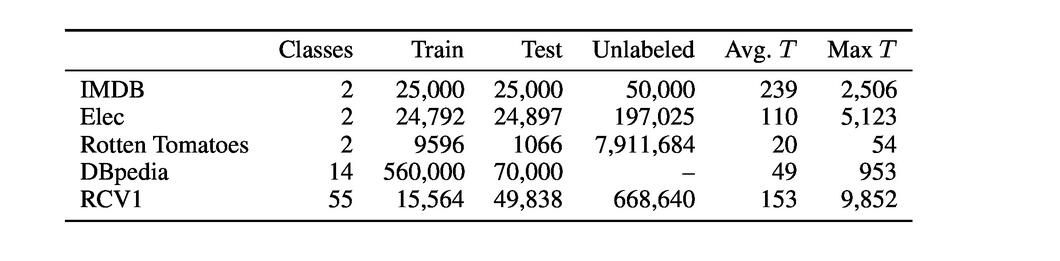
\includegraphics[width=.9\linewidth]{dataset.jpg}
		\end{figure}
	\end{columns}
\end{frame}

\begin{frame}{No Overfit}
	\begin{columns}[onlytextwidth]
		
		\column{1.2\textwidth}
		\begin{figure}
			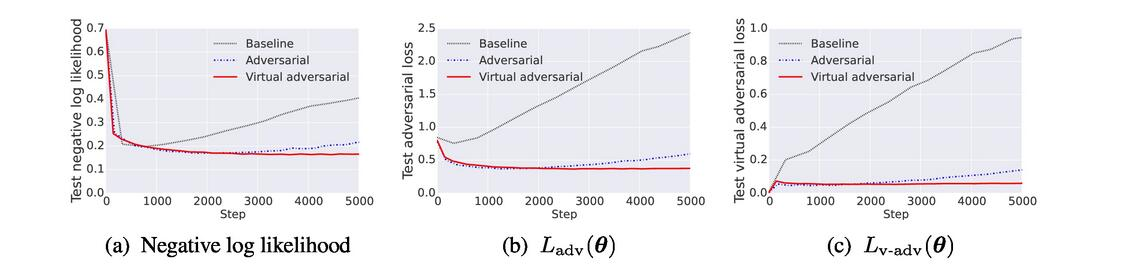
\includegraphics[width=.9\linewidth]{quxian.jpg}
		\end{figure}
	\end{columns}
\end{frame}

\begin{frame}{Result to IMDB}
	\begin{columns}[onlytextwidth]
		
		\column{.9\textwidth}
		\begin{figure}
			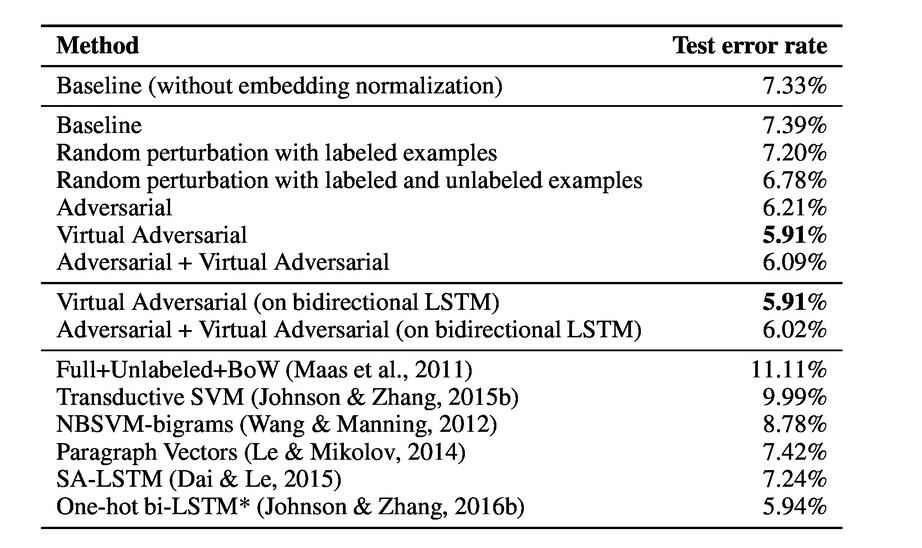
\includegraphics[width=.9\linewidth]{imdb.jpg}
		\end{figure}
	\end{columns}
\end{frame}

\begin{frame}{Good or Bad?}
	\begin{columns}[onlytextwidth]
		
		\column{1\textwidth}
		\begin{figure}
			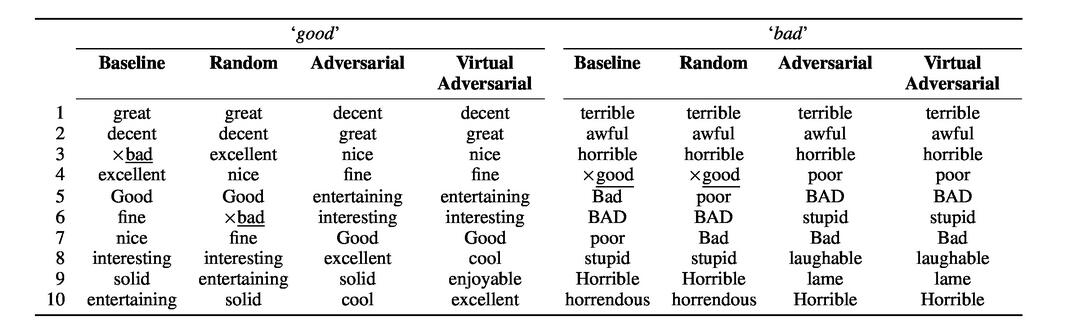
\includegraphics[width=1\linewidth]{goodbad.jpg}
		\end{figure}
	\end{columns}
\end{frame}

\begin{frame}{Results on Elec and RCV1}
	\begin{columns}[onlytextwidth]
		
		\column{1\textwidth}
		\begin{figure}
			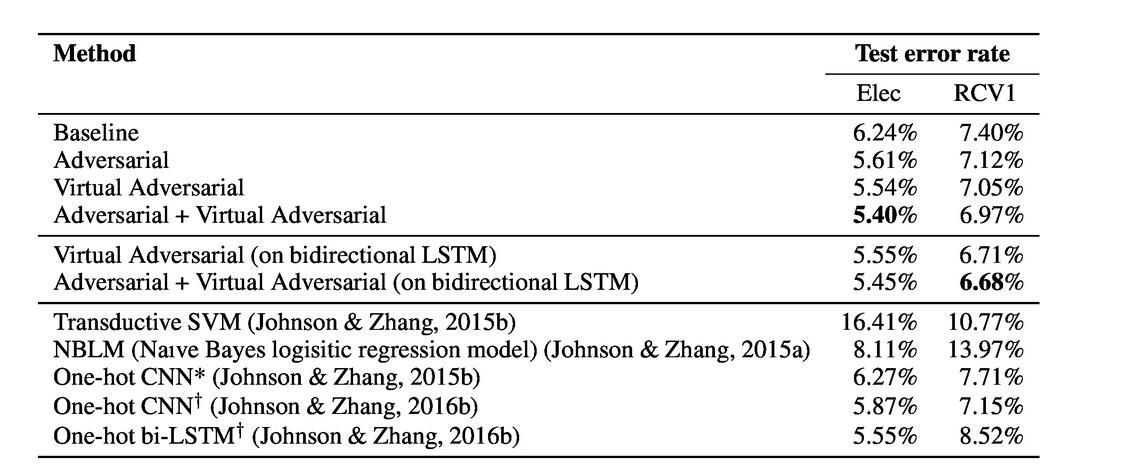
\includegraphics[width=1\linewidth]{elec.jpg}
		\end{figure}
	\end{columns}
\begin{itemize}
	\item $*$ indicates using pretrained embeddings of CNN, and $\dag$ indicates using pretrained embeddings of CNN and bidirectional LSTM
	\end{itemize}
\end{frame}

\begin{frame}{Thanks to \LaTeX\quad and mtheme}
	
	Get the source of this theme and the demo presentation from
	
	\begin{center}\url{github.com/matze/mtheme}\end{center}
	
	The theme \emph{itself} is licensed under a
	\href{http://creativecommons.org/licenses/by-sa/4.0/}{Creative Commons
		Attribution-ShareAlike 4.0 International License}.
	
	\begin{center}\ccbysa\end{center}
	
\end{frame}

\begin{frame}{OpenSource}
	
	Get the source code of this slide from
	
	\begin{center}\url{github.com/lwshanbd/bigdata_slide}\end{center}
	

	
\end{frame}